\documentclass[11pt,letterpaper]{article}
\usepackage[pdftex]{graphicx}
\usepackage[noload]{qtree}

\begin{document}

\title{CS542 (Fall 2021) Written Assignment 3 \\ Statistical Parser: CKY Algorithm\footnote{This assignment is adapted from Hal Daume's.}}
\author{Due November 7, 2021}
\date{}
\maketitle

\section*{Assignment}

You are given a small grammar on the next page. Your task is to use the probabilistic CKY algorithm to fill in the \textit{table} and \textit{back} arrays for the two sentences ``time flies like an arrow" and ``fruit flies like a banana". Please also draw the final tree for each sentence. Note that because the grammar is not in Chomsky normal form (it contains unary rules), you will need to modify the algorithm in Figure C.3 of the Jurafsky and Martin book to handle the unary rules.\\

\noindent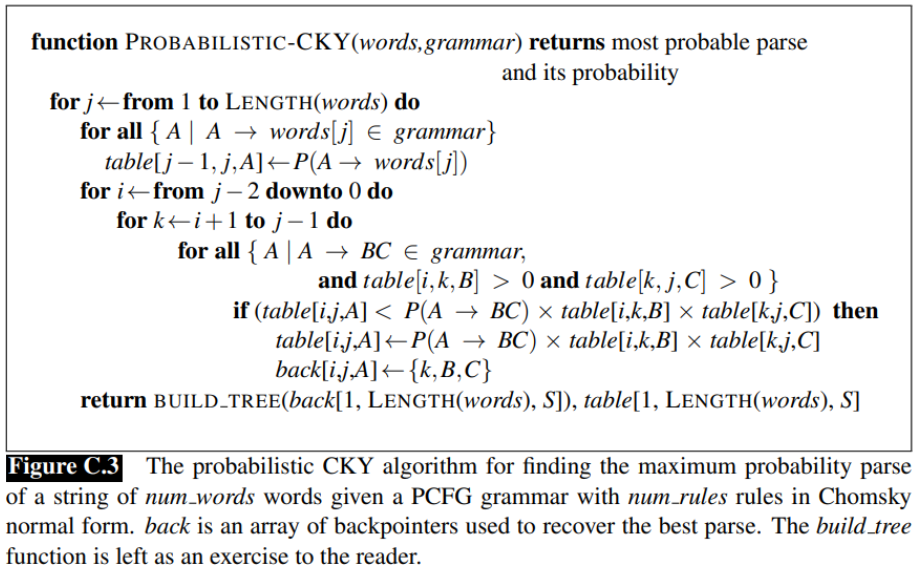
\includegraphics[width=358px]{figure_c_3.png}

\subsection*{Grammar}

\begin{verbatim}
S       -> NP VP      [0.5]
S       -> VP         [0.2]
S       -> NP VP_PP   [0.2]
S       -> VP PP      [0.1]
VP_PP   -> VP PP      [1.0]
NP      -> DT NN      [0.5]
NP      -> Nominal NN [0.2]
NP      -> NN         [0.3]
VP      -> VB NP      [0.6]
VP      -> VB PP      [0.2]
VP      -> VB NP_PP   [0.1]
VP      -> VB         [0.1]
NP_PP   -> NP PP      [1.0]
PP      -> IN NP      [1.0]
DT      -> 'a'        [0.5]
DT      -> 'an'       [0.5]
NN      -> 'time'     [0.2]
NN      -> 'flies'    [0.2]
NN      -> 'arrow'    [0.2]
NN      -> 'fruit'    [0.2]
NN      -> 'banana'   [0.2]
VB      -> 'time'     [0.3]
VB      -> 'flies'    [0.4]
VB      -> 'like'     [0.3]
IN      -> 'like'     [1.0]
Nominal -> 'fruit'    [1.0]
\end{verbatim}\newpage

\section*{Submission Instructions}

Please submit your solutions (in PDF format) to the submission box on Canvas. If you are familiar with \LaTeX, you may use the table and tree templates below (see {\tt HW3.tex}, which is downloadable from Canvas). Alternatively, you may draw your tables and trees by hand and scan them into a PDF.\\

\begin{tabular}{|c|c|c|c|c|}

\multicolumn{1}{c}{time} & \multicolumn{1}{c}{flies} & \multicolumn{1}{c}{like} & \multicolumn{1}{c}{an} & \multicolumn{1}{c}{arrow} \\ 
\hline 
• & • & • & • & • \\ 
\hline 
\multicolumn{1}{c|}{} & • & • & • & • \\ 
\cline{2-5} 
\multicolumn{2}{c|}{} & • & • & • \\ 
\cline{3-5} 
\multicolumn{3}{c|}{} & • & • \\ 
\cline{4-5} 
\multicolumn{4}{c|}{} & • \\ 
\cline{5-5} 
\end{tabular} \\\\

\Tree[.A [.B [.D ... ]
             [.E ... ]]
         [.C [.F ... ]
             [.G [.H ... ]
                 [.I ... ]]]]
                 
\end{document}